\documentclass{standalone}
\usepackage[T1]{fontenc}
\usepackage{mathptmx}
\usepackage{pgfplots}
\pgfplotsset{compat=1.18}
\begin{document}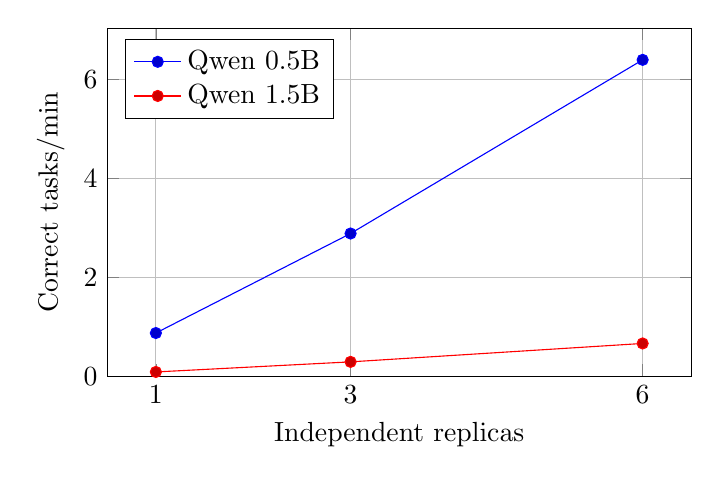
\begin{tikzpicture}
\begin{axis}[width=9cm,height=6cm,xlabel={Independent replicas},ylabel={Correct tasks/min},xtick={1,3,6},ymin=0,grid=major,legend pos=north west]
\addplot+[mark=*] coordinates {(1,0.8713) (3,2.8831) (6,6.3930)};\addlegendentry{Qwen 0.5B}
\addplot+[mark=*] coordinates {(1,0.0847) (3,0.2886) (6,0.6607)};\addlegendentry{Qwen 1.5B}
\end{axis}\end{tikzpicture}\end{document}
